% !TEX TS-program = pdflatex
% !TEX encoding = UTF-8 Unicode

%\documentclass[ing,male,java,dept460,oneside]{diploma}
\documentclass{article}

\usepackage[czech]{babel}
\usepackage[T1]{fontenc}
\usepackage[utf8]{inputenc}
\usepackage{color}
\usepackage{geometry}
\usepackage{float}
\usepackage{graphicx}
\usepackage[stable]{footmisc}
\usepackage{hyperref}
\usepackage{amsfonts}
 \usepackage{bbm}
 \usepackage{booktabs}
 \usepackage{url}
 \usepackage{nameref}



% \ThesisAuthor{Josef Raška}

% U bakalarske praxe neni nutne nazev zadavat
%\ThesisTitle{Tos ten android ze}

% U bakalarske prace neni nutne anglicky nazev zadavat
%\EnglishThesisTitle{The Android stuff}

%\SubmissionDate{29. dubna 2016}

%\PrintPublicationAgreement{true}


%\Thanks{Podekovani \newline Dalsi lajna }


%\CzechAbstract{Cesky abstrakt}

%\CzechKeywords{vlastní číslo, vlastní vektor, vlastní dvojice, aplikace vlastních čísel, mocninná metoda, Lanczosova metoda, předpodmínění}

%\EnglishAbstract{English abstract}

%\EnglishKeywords{Android, development}

\title{Diplomová práce}
\author{Josef Raška \(ras0029\)}
\newtheorem{priklad}{Příklad}[section]
\newtheorem{veta}{Věta}[section]
\newtheorem{alg}{Algoritmus}[section]

\newcommand{\usecase}[2]{\paragraph{#1}\label{#2}\mbox{}\\ \newline \noindent}

\begin{document}
%\maketitle
%\MakeTitlePages
\urlstyle{same}

\tableofcontents
\listoffigures
\listoftables
%\lstlistoflistings

\newpage

\section{Úvod}

\section{Návrh aplikace}
\subsection{Popis aktérů}
\begin{figure}[H]
        \centering
                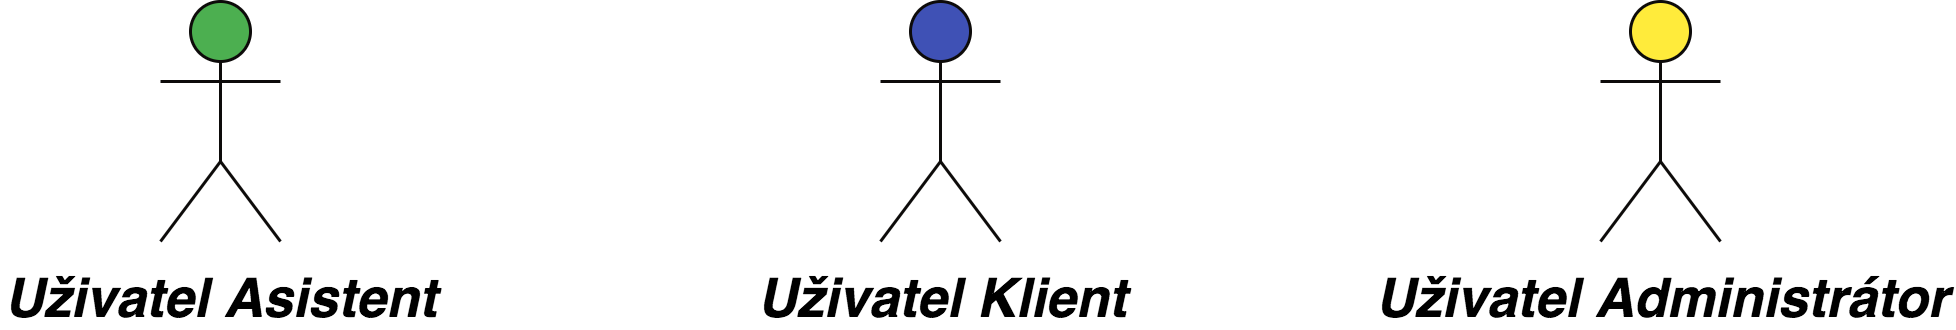
\includegraphics[scale=0.15]{img/actors.png}
        \caption{Aktéři systému}
        \label{fig:actors}
\end{figure}

\subsubsection{Uživatel Asistent}
Jedná se o aktéra, který je zároveň klientovi s mentálním postižením odborným asistentem,
jenž o něj pečuje a poskytuje mu podporu. Tento aktér je releventní k vytváření obsahu,
který má pomoci klientovi k lepší orientaci při cestování a také mu může připravenou
cestu předvést. Může také nahraná data editovat a případně je rozšiřovat. Může také zadat
do aplikace zadat své kontaktní údaje pro možnou nečekanou situaci klienta na cestách, případně
nastavit zálohování uložených dat pro zamezení jejich ztráty při ztrátě telefonu nebo jeho výměně
za jiný.

\subsubsection{Uživatel Klient}
Klient je osoba pro kterou je aplikace primárně určena a má mu pomoci vyřešit problém,
v tomto případě pomoci z orientací při cestování. Může si prohlížet obsah a zejména ho
využívat při cestách v terénu. Uživatel by měl být upozorněn na všechny uložené a rozeznané
data v závisloti na své pozici a měl by tak získat releventní informace k tomu, kde se právě
nachází. Dále může aplikaci využít ke snadnému kontaktování svého asistenta.

\subsubsection{Uživatel Administrátor}

\subsection{Use casy}
\label{labelx}
Pro uživatele klienta i asistenta jsou definovány případy užití zvlášť, neboť se celé chodvání
a použití aplikace bude v obou případech značně lišit.

\subsubsection{Uživatel asistent}
Pro uživatele asistnta jsou určeny složitější operace pro vytváření interaktivního obsahu pro klienta,
nastavování aplikace a prezentace klientovi. Pro use casy asistenta platí, že klient může těmto
krokům přihlížet, pokud o to projeví zájem.

\begin{figure}[H]
        \centering
                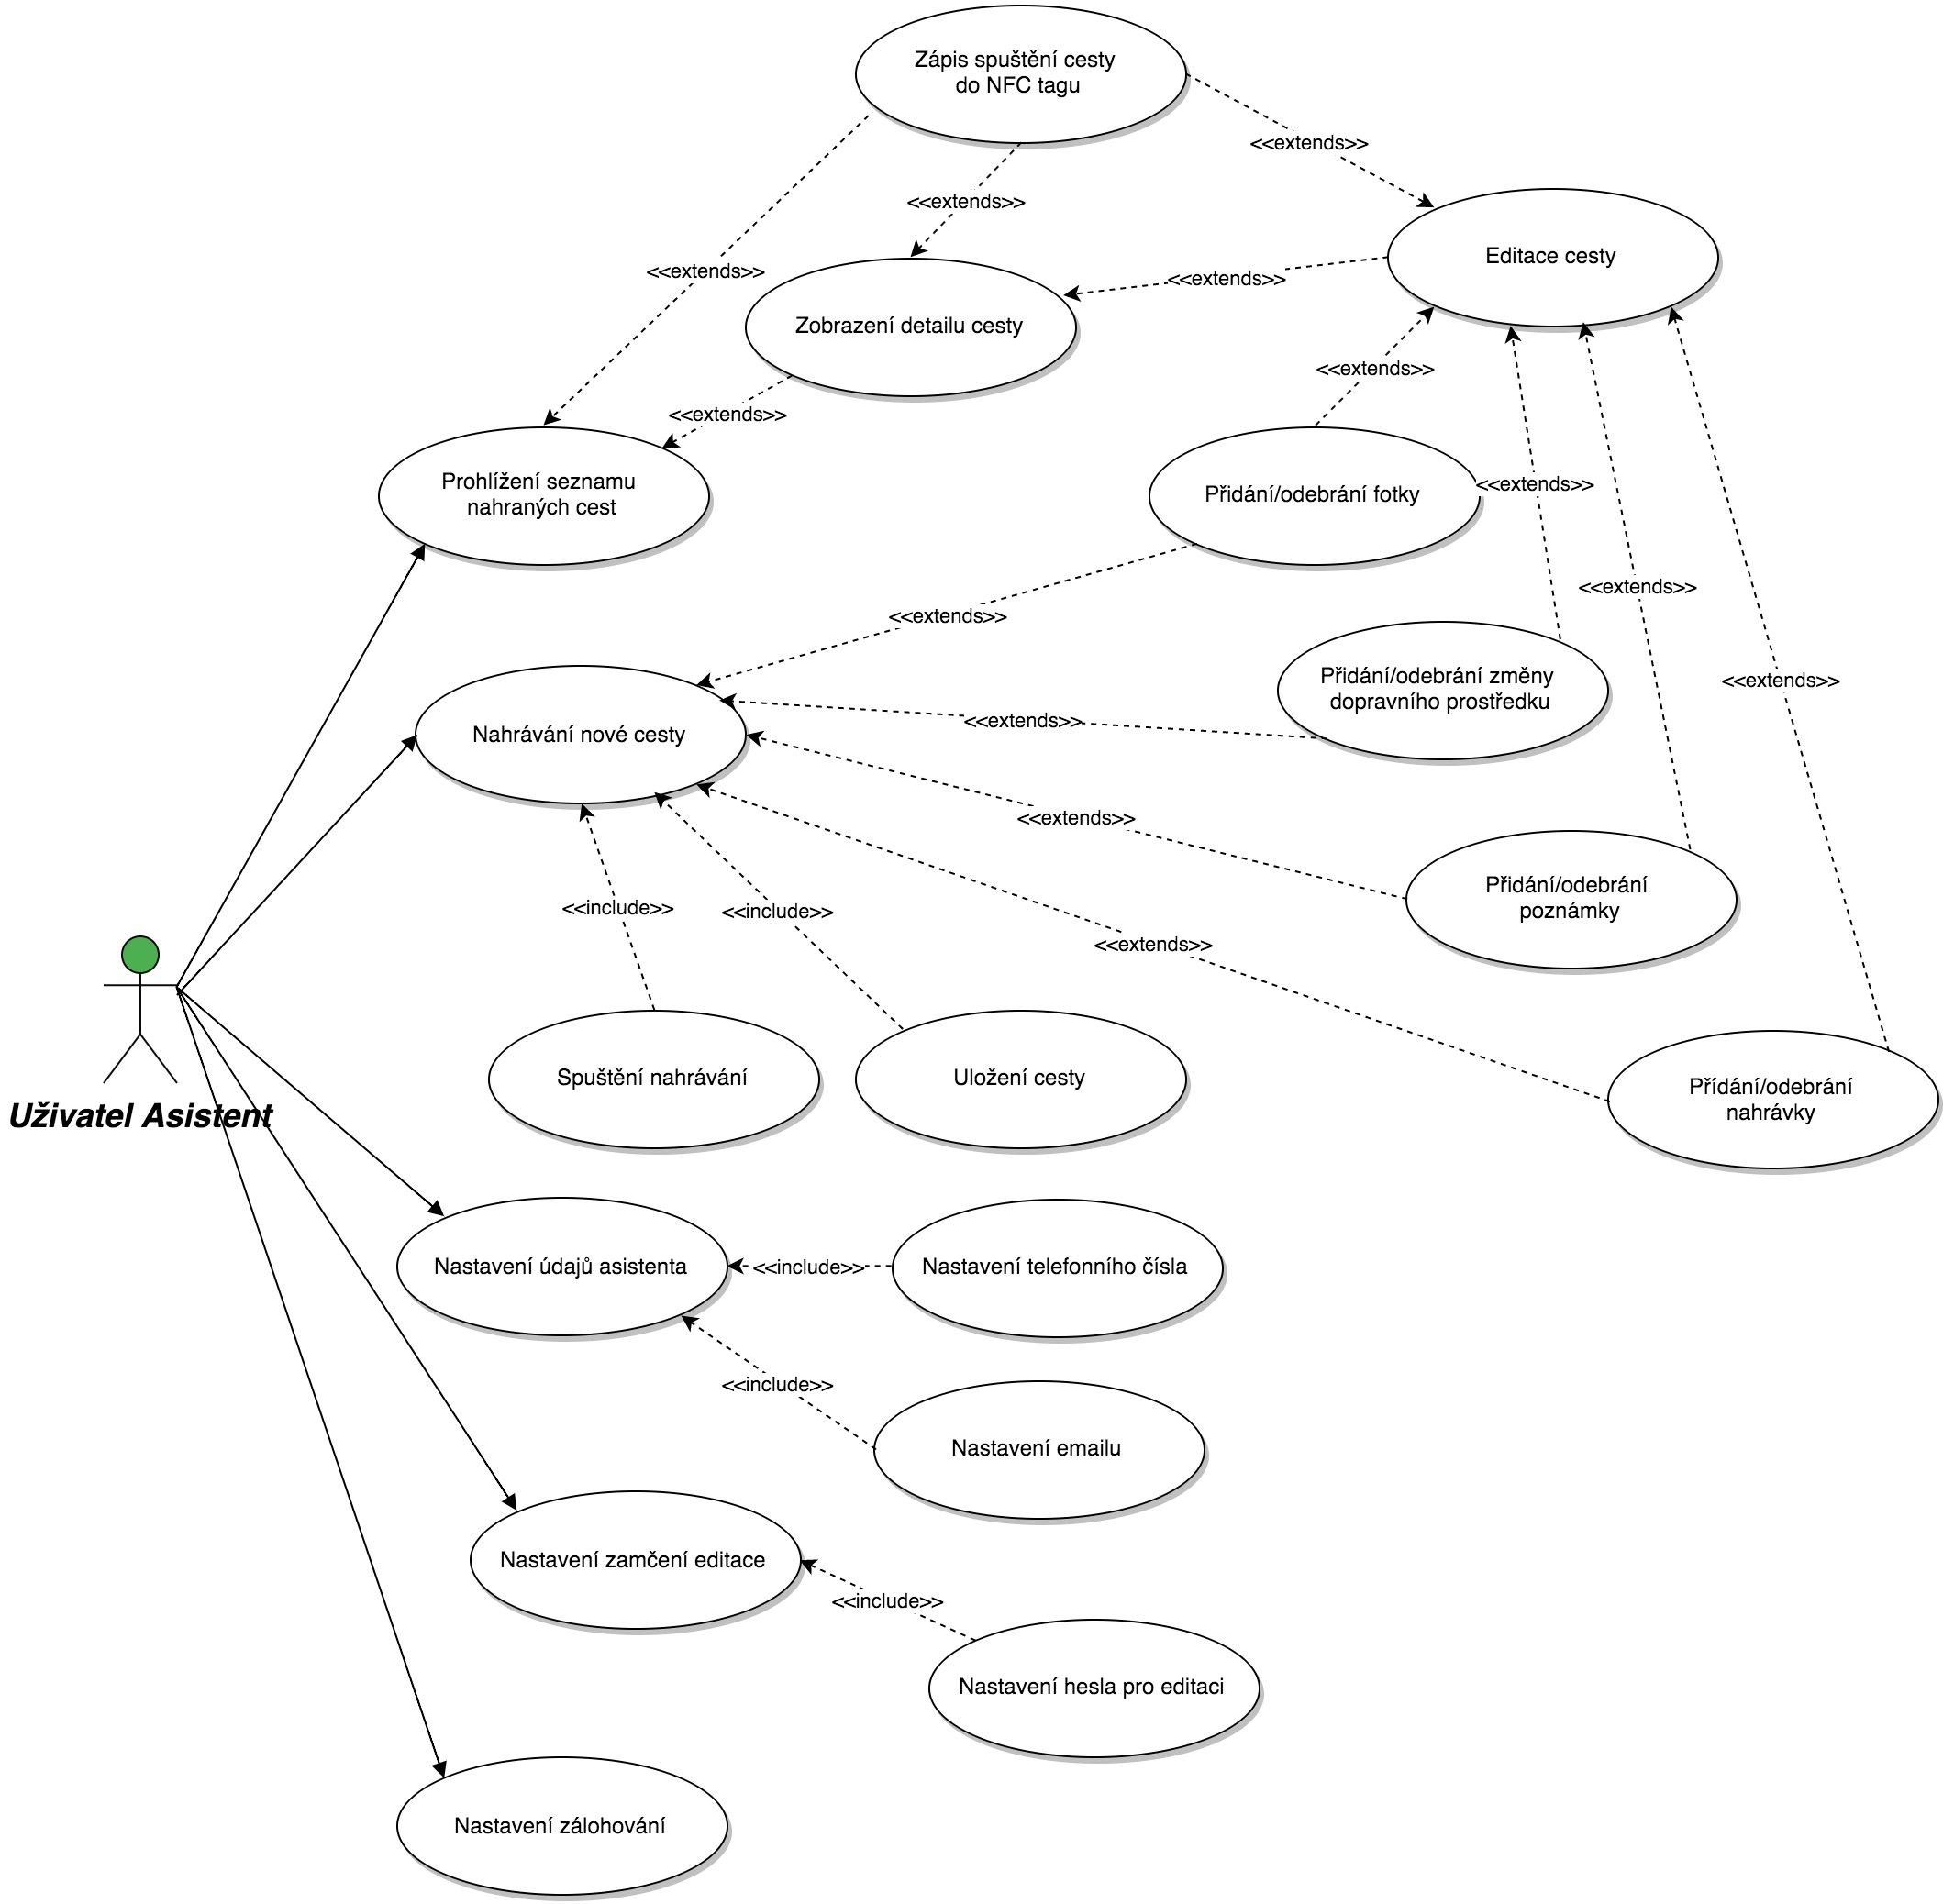
\includegraphics[scale=0.2]{img/UseCasesAsistant.png}
        \caption{Diagram use casů uživatele asistent}
        \label{fig:UseCasesAsistant}
\end{figure}
%
%\usecase{name}{label}
%\textbf{Aktéři:} Asisitent
%
%\vspace{0.1cm}
%\noindent
%\textbf{Hlavní scénář:}
%
%\vspace{0.1cm}
%\noindent
%\textbf{Prekondice:}
%
%\vspace{0.1cm}
%\noindent
%\textbf{Spouštěč:}
%
%\vspace{0.1cm}
%\noindent
%\textbf{Rozšíření:}

\usecase{Prohlížení seznamu nahraných cest}{prohizeniasistent}
\textbf{Aktéři:} Asisitent

\vspace{0.1cm}
\noindent
\textbf{Hlavní scénář:} Na úvodní obrazovce jsou zobrazeny všechny dosud nahrané cesty ve seznamu pod sebou.
Lze vidět pouze základní údaje a přiřazený obrázek pro snadnou orientaci. Uživatel se pomocí
kliknutí na řádek může podívat na celý detail cesty, případně pomocí rychlých akcí spustit ihned asistenci
a podobně.

\vspace{0.1cm}
\noindent
\textbf{Spouštěč:} Uživatel spustí aplikaci nebo se do ní vrátí pomocí notifikace v notifikační liště.

\vspace{0.1cm}
\noindent
\textbf{Rozšíření:}
\begin{itemize}
  \item \nameref{detailasistent}
  \item \nameref{nfczapis}
\end{itemize}


\usecase{Zobrazení detailu cesty}{detailasistent}
\textbf{Aktéři:} Asisitent

\vspace{0.1cm}
\noindent
\textbf{Hlavní scénář:} Uživateli se zobrazí detail cesty se všemi informacemi, ktré jsou o ní uloženy.
Na mapě si může prohlédnout kudy vedla, an místech fotografií jsou miniatury fotek, při změně dopravních
prostředků lze vidět ikony daných prostředků, zvukově a textové záznamy jsou označeny příslušnou ikonou.
Při klepnutí na indikátor některého z těchto záznamů se zobrazí jeho popis, který uživatel dříve zadal.
V detailu cesty lze poklepáním na tlačítko editovat přejít do módu editace cesty a všechny dříve zmíněné
záznamy upravit

\vspace{0.1cm}
\noindent
\textbf{Prekondice:} Cesta je uložena.

\vspace{0.1cm}
\noindent
\textbf{Spouštěč:} Uživatel klepne na řádek se zobrazenou cestou v seznamu cest.

\vspace{0.1cm}
\noindent
\textbf{Rozšíření:}
\begin{itemize}
  \item \nameref{editacecesty}
  \item \nameref{nfczapis}
\end{itemize}

\usecase{Zapsání cesty do NFC tagu}{nfczapis}
\textbf{Aktéři:} Asisitent

\vspace{0.1cm}
\noindent
\textbf{Hlavní scénář:} Uživateli se zobrazí
obrazovka, která jej instruuje k přiložení NFC tagu k telefonu. Jakmile telefon zaznamená blízkost tagu,
zapíše do něj informaci o uložené cestě pro následné rychlé spouštění při přiložení tagu k telefonu.

\vspace{0.1cm}
\noindent
\textbf{Prekondice:} Cesta je uložena.

\vspace{0.1cm}
\noindent
\textbf{Spouštěč:} Uživatel klepne na ikonu NFC v detailu cesty nebo an rozšiřující menu v seznamu cest.


\usecase{Editace cesty}{editacecesty}
\textbf{Aktéři:} Asisitent

\vspace{0.1cm}
\noindent
\textbf{Hlavní scénář:} Uživatel může editovat všechny uložné informace o cestě. Přepsání editačních
polí může změnit názvy a popis nahrané cesty, podržením a přetažením miniatur fotek nebo ikon dalších údajů na mapě může změnit
jejich pozici a tudíž místo, kdy se později vyvolají. Dále může podržením přetažením měnit tvar trasy,
při klepnutí na mapu přidat další záznamy. Jakmile je uživatel s editací spokojen, klepnutím na tlačíko
uložit se údaje zapíší do databáze a následující asistence cestování bude tyto údaje používat.

\vspace{0.1cm}
\noindent
\textbf{Prekondice:} Cesta je uložena.

\vspace{0.1cm}
\noindent
\textbf{Spouštěč:} Uživatel klepne na tlačítko editovat v detailu cesty.

\vspace{0.1cm}
\noindent
\textbf{Rozšíření:}
\begin{itemize}
  \item \nameref{pridanifotky}
  \item \nameref{pridaninahravky}
  \item \nameref{pridanipoznamky}
  \item \nameref{pridanizmenyprostredku}
\end{itemize}

\usecase{Přídání fotky}{pridanifotky}
\textbf{Aktéři:} Asisitent

\vspace{0.1cm}
\noindent
\textbf{Hlavní scénář:} Spustí se fotoaparát zařízení a uživatel může začít fotit. Jakmile pořídí
fotografii, zobrazí se v aplikace okno pro zadání názvu fotky s dotazem pro uložení. Uživatel zadá název
a klepnutím na potvrzovací tlačítko se fotka uloží mezi data aplikace a zobrazí mezi aktuálními fotografiemi
na místě polohy uživatele v době pořízení fotografie.
\vspace{0.1cm}
\noindent
\textbf{Prekondice:} Uživatel nahrává nebo edituje cestu

\vspace{0.1cm}
\noindent
\textbf{Spouštěč:} Uživatel klepl na tlačítko přidat fotku

\usecase{Přídání zvukové nahrávky}{pridaninahravky}
\textbf{Aktéři:} Asisitent

\vspace{0.1cm}
\noindent
\textbf{Hlavní scénář:} Uživateli se zobrazí obrazovka s textem mluvte a zvuk se zaznamenává.
Když je uživatel hotov, klepne na tlačítko stop a může nahrávce přidat název, který se bude později zobrazovat.
Poté tlačítkem nahrávku uloží mezi data aplikace s přiřazenou aktuální polohou uživatele.

\vspace{0.1cm}
\noindent
\textbf{Prekondice:} Uživatel nahrává nebo edituje cestu

\vspace{0.1cm}
\noindent
\textbf{Spouštěč:} Uživatel klepl na tlačítko přidat nahrávku

\usecase{Přídání poznámky}{pridanipoznamky}
\textbf{Aktéři:} Asisitent

\vspace{0.1cm}
\noindent
\textbf{Hlavní scénář:} Uživateli se zobrazí okno s textovým vstupem a vysune se klávesnice. Uživatel
zadá textovou poznámku a po klepnutí na potvrzovací tlačítko se poznámka uloži s asociací k aktuální poloze
uživatele.

\vspace{0.1cm}
\noindent
\textbf{Prekondice:} Uživatel nahrává nebo edituje cestu

\vspace{0.1cm}
\noindent
\textbf{Spouštěč:} Uživatel klepl na tlačítko přidat poznámku

\usecase{Přídání změny dopravního prostředku}{pridanizmenyprostredku}
\textbf{Aktéři:} Asisitent

\vspace{0.1cm}
\noindent
\textbf{Hlavní scénář:} Zobrazí se okno se nabídkou tlačítek s obrázkem dopravního prostředku.
Uživatel může zároveň přidat ke změně dopravního prostředku přidat popis. Po kliknutí na
tlačítko s dopravním prostředkem se změna dopravního prostředku uloží s asociovanou aktuální polohou
uživatele.

\vspace{0.1cm}
\noindent
\textbf{Prekondice:} Uživatel nahrává nebo edituje cestu

\vspace{0.1cm}
\noindent
\textbf{Spouštěč:} Uživatel klepl na tlačítko s aktuálním dopravním prostředkem




\subsubsection{Uživatel klient}
Pro klienta jsou určeny více intuitivní a nenáročné operace vyžadující co nejméně aktivních
kroků z klientovi strany. Aplikace by měla na základě polohy a dalších údajů sama rozpoznat,
co má v  danou chvíli udělat.

\begin{figure}[H]
        \centering
                \includegraphics[scale=0.2]{img/UseCasesClient.png}
        \caption{Diagram use casů uživatele klient}
        \label{fig:UseCasesClient}
\end{figure}










\subsection{Použité nástroje}
\subsubsection{draw.io (http://www.draw.io)}
Online nástroj pro tvorbu grafů, všech různých typů diagramů, myšlenkových map a dalších.
Celý edior běží pouze v prohlížeči a synchronizuje vytvářené grafy s připojeným úložištěm
Google Drive nebo Dropbox. Grafy jsou tak přístupné  a editovatelné odkudkoliv a aplikace
je opravdu pokročilá a při práci není vůbec poznat, že vše probíhá pouze v prohížeči.
Umožňuje sdílení i export zhotovených diagramů do mnoha formátů a je tedy velice snadné
sdílet a používat vytvořenou práci.
Nástroj byl použit pro vytváření use case diagramů a třídnách diagramů v této práci.
\begin{figure}[H]
        \centering
                
\includegraphics[scale=0.2]{img/drawiologo.png}
        \caption{Logo nástroje draw.io}
        \label{fig:iologo}
        \centering Zdroj: \url{http://www.draw.io}
\end{figure}

%\subsection{Podnadpis\footnote{Inspirace v \cite{saad}}}



\section{Závěr}


\begin{thebibliography}{99}

\end{thebibliography}

  \appendix

  \section{Zdrojové kódy}
  Kódy lze nalézt i na přiloženém CD.

\end{document}